\label{ch:six}
Towards the end of the project we decided to implement a python module to do testing and analysis on some candidate probability distributions. The motivation for this was given mainly by the results showed again in \cite{RW03}. 
\section{Analysis design and goals}
    To visualize and motivate the scope of this analysis we expand Eq. \ref{eq:bounds} as follow
    \begin{equation}
    	\keyrate{X}{Y}{Z} \leq \redintrinfo{X}{Y}{Z} \leq \intrinfo{X}{Y}{Z} \leq I_{form} (X;Y|Z)
    \end{equation}
    including also the information of formation.
    As mentioned before, obtaining a value for the secret-key rate and information of formation --- the fundamental quantities for key agreement --- requires a \textit{possible} protocol. 
    For their bounds (i.e. the central parts of the inequality) we can obtain direct numerical values from the probability distribution alone. 
    The aim of this part of the project is then to take a candidate as given in Fig. \ref{Tab:candidate2} and trace the values of the reduced and normal intrinsic information for  variation of the probability distribution.\\
    
    A good result we hope to obtain is a probability distribution for which the reduced measure tends to $0$, while the intrinsic information remains larger than $0$, bounding also the information of formation to be greater than $0$. 
    Due to the tightness of the bounds, this will constrain the value for the secret key rate down to (possibly) $0$, while keeping a non-zero key cost ($I_{\text{form}}$).
    This will lead to a new candidate for bound information.\\
    
    In order to perform analysis on those measures we firstly had to implement a library of modules that dealt with the probability and information theory aspects.
    Following criteria for separability of quantum states, a quantum mechanics module was also implemented to translate and later tests the distributions from the quantum to classical regime.
    The intrinsic information (and its reduced counterpart) is defined as an \emph{infimum} over the set of tripartite probability distributions. 
    To find a correct value it would require to solve an optimization problem. 
    The definition given in section \ref{intrininfo} however does not allow us to formulate the problem as convex, or, at least, not a trivial one, since the mutual information is only convex for a fixed term.
    We decided then to adopt a Monte-Carlo method to estimate them.
     
    For each step --- i.e. for each variation --- of the candidate base probability, the values of 
    \begin{itemize}
    	\item	mutual information
    	\item	intrinsic information
    	\item	reduced intrinsic information
    	\item	trace over quantum state witness given in \cite{DPS04}
    \end{itemize}
    are estimated.
\section{Different noises analysis}

	\begin{figure}[h!]
		\centering
		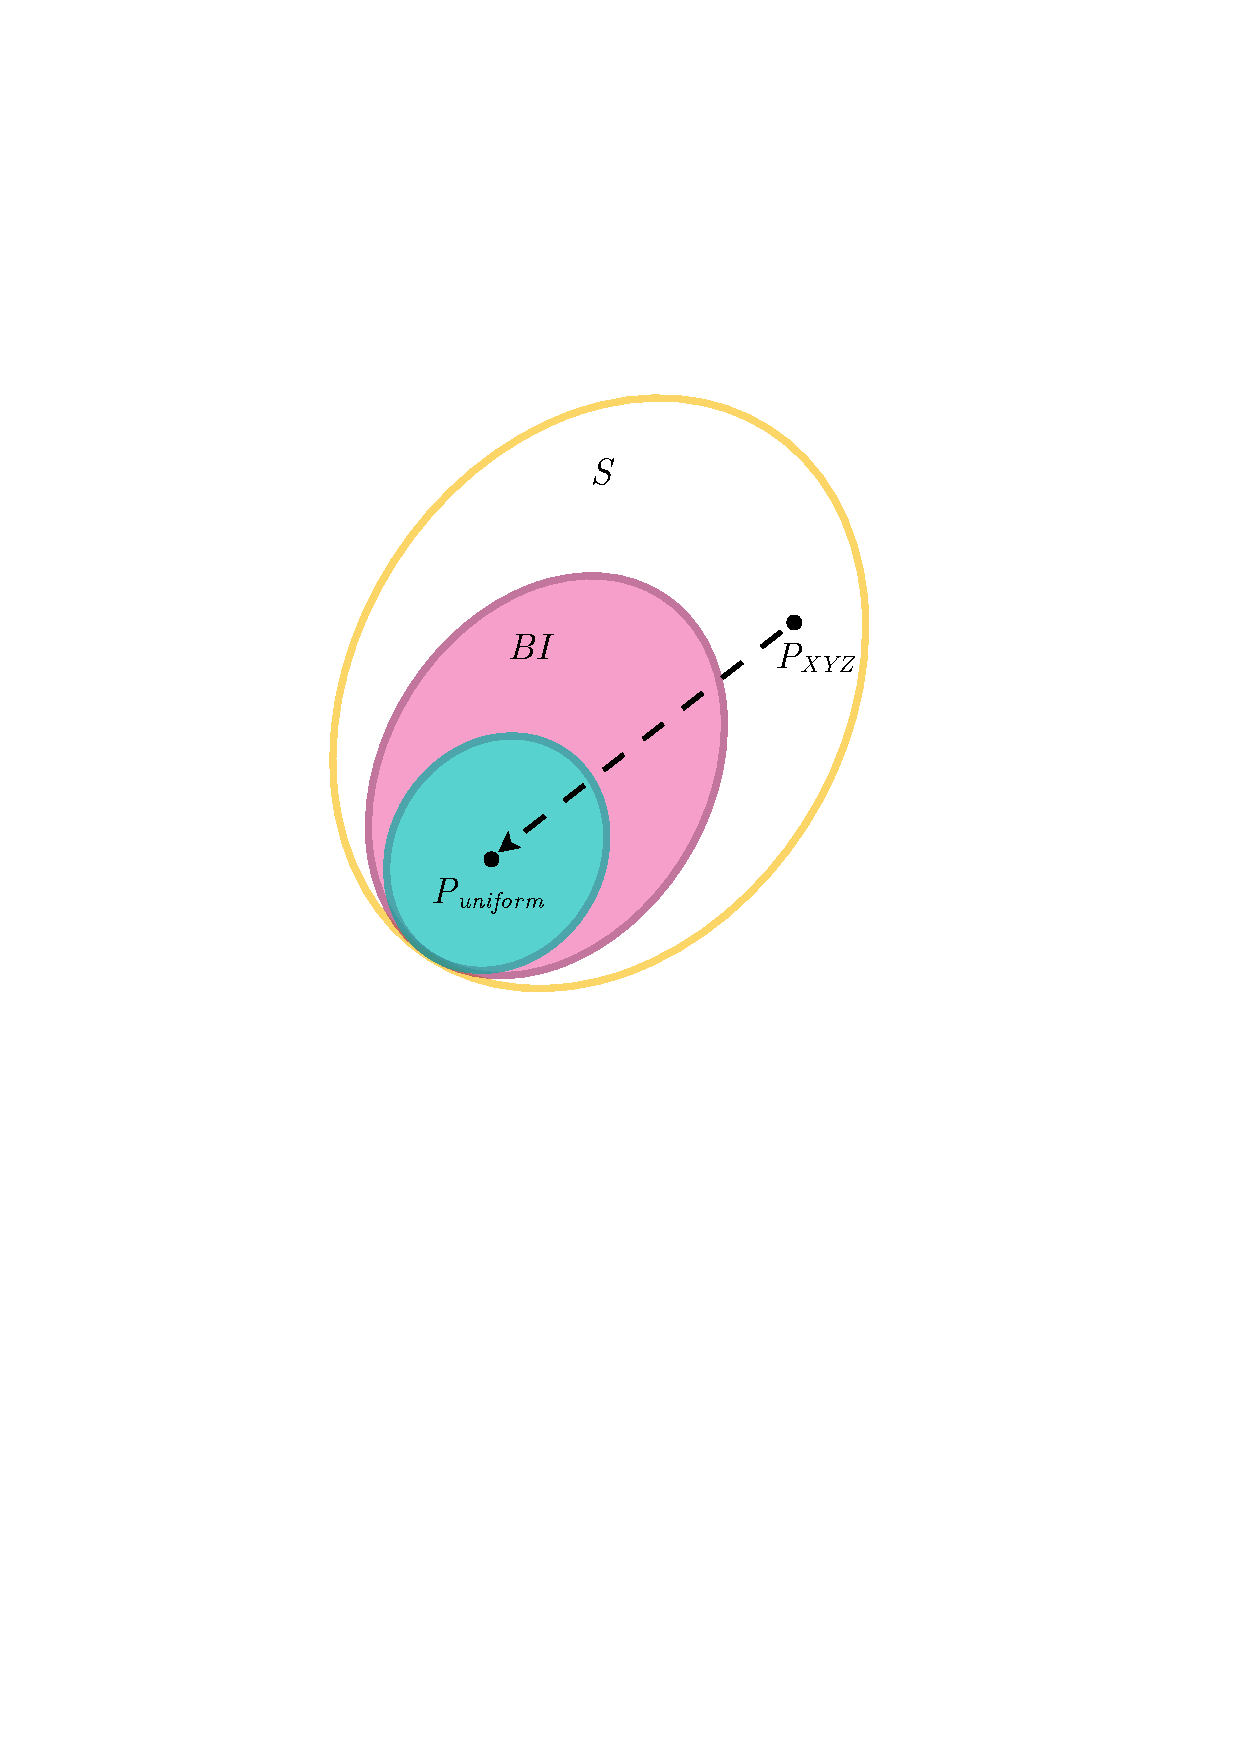
\includegraphics[scale=0.5]{images/analysis-path}
		\caption{From the set $S$ of tripartite distributions we create a "path"
towards distributions with zero key cost (cyan), going through the ones without extractable key (magenta). The distributions that holds bound information reside in the cyan$\setminus$magenta part.}
		\label{Fig:analysis-path}
	\end{figure}
	The variations of the distribution mentioned above are linear steps toward a noise distribution we define.
	The first and obvious noise function we tested is the uniform distribution, which acts on all values of $P_{XYZ}$.
	Following the idea of the candidate distribution showed in Fig. \ref{Tab:candidate2} we  also utilized a noise function that operates on the non-correlated part for Alice and Bob.
	
	This method of simulating noise added to a known distribution takes also inspiration from the quantum world. 
	A method to look for bound entangled states applies a noise channel to a known entangled state and then the new state is tested on different separability criteria.
	The intuition comes from the respectively enclosed convex sets of separable states.
	
	 
	\begin{figure}
		\begin{subfigure}{0.5\textwidth}
			%Noise 1

		\begin{center}
		\begin{tabular}{|l r||c|c|c|c|}
		    \hline 
		    		 &	$X$ & $0$ & $1$ & $2$ & $3$ \\ 
		    $Y$ &		  &		&			&			&		\\
		    \hline 
		    \hline
		    $0$ &		   & $0$ & $0$ & $a$ & $a$ \\ 
		    \hline 
		    $1$ &		   & $0$ & $0$ & $a$ & $a$ \\ 
		    \hline 
		    $2$ &		   & $a$ & $a$ & $0$ & $0$ \\ 
		    \hline 
		    $3$ &		   & $a$ & $a$ & $0$ & $0$ \\ 
		    \hline 
		  \end{tabular} 
	\end{center}
			\subcaption{Noise1}
			\label{Fig:noise1}
		\end{subfigure}
		\begin{subfigure}{0.5\textwidth}
			%Noise 2

		\begin{center}
		\begin{tabular}{|l r||c|c|c|c|}
		    \hline 
		    		 &	$X$ & $0$ & $1$ & $2$ & $3$ \\ 
		    $Y$ &		  &		&			&			&		\\
		    \hline 
		    \hline
		    $0$ &		   & $a$ & $a$ & $a$ & $a$ \\ 
		    \hline 
		    $1$ &		   & $a$ & $a$ & $a$ & $a$ \\ 
		    \hline 
		    $2$ &		   & $a$ & $a$ & $0$ & $0$ \\ 
		    \hline 
		    $3$ &		   & $a$ & $a$ & $0$ & $0$ \\ 
		    \hline 
		  \end{tabular} 
	\end{center}
			\subcaption{Noise2}
			\label{Fig:noise2}
		\end{subfigure}
		\caption{Different noises disturbs different parts of the correlation between $X$ and $Y$}
		\label{Fig:noises}
	\end{figure}
	
\section{The problem with the reduced intrinsic information}\label{problem}
    During the implementation of the module we were confronted with some issues on the measure of the reduced intrinsic information.
    Recalling Eq. \ref{eq:reducedintrinfo}, we first generate random channels $XYZ \rightarrow U$ to get the conditional probability $P_{U|XYZ}$. 
%    In some cases, also a channel $X\rightarrow U$, or $XY \rightarrow U$ can be used.
    Then the intrinsic information is minimized over all possible channels $ZU \rightarrow \bar{ZU}$.
    Ideally, we want to show how the reduced intrinsic information goes to $0$, so that the secret key rate also falls to $0$. 
    Thus, $\Ent (U)$ is a lower bound on the value of the reduced intrinsic information.
    Since $U$ is generated through an arbitrary channel, however, it will not have $\Ent (U) = 0$.
    In order to minimize this lower bound, the marginal $P_U$ should be deterministic.
    
    Observing this, we questioned the usefulness of the reduced intrinsic information as a measure to demonstrate the existence of bound information, contrary to we thought at the beginning. 
    
\section{Results}
Despite the difficulties encountered in implementing the code, we were able to produce some marginal results.
When the noise functions were applied to the marginal $P_{XYZ}$ of the distribution in Fig. \ref{Tab:candidate} we were able to make the following observations
\begin{itemize}
\item For the uniform noise, as expected, the behaviour presents no intrinsic information nor reduced intrinsic information. The two measures remain the same until around $\alpha = 1- 1/8 = 0.875$. Around that point the reduced intrinsic information of the behaviour \textit{decrases} until reaching $1$, as we already knew from \cite{RW03}.

\item For the noise in Fig. \ref{Fig:noise1}, we notice first of all that the intrinsic information is not monotonic along the path. It takes the form of a convex function with minimum for an $\alpha$ around $0.4$. At both ends of the path the two measures diverge resulting in $\intrinfo{X}{Y}{Z} \approx 1$ and $\redintrinfo{X}{Y}{Z} \approx 0.5$ for $\alpha = 0$, i.e. for just the noise function represented in the figure. On the other end we obtain again the results as before for the marginal of the candidate.

\item Finally for the noise function in fig. \ref{Fig:noise2} we observe the same general behaviour as before. 
The observable minimum is around values $\alpha = 0.2$ and for just the noise function the reduced intrinsic information falls to about $\redintrinfo{X}{Y}{Z} \approx 0.125$ and $\intrinfo{X}{Y}{Z} \approx 0.25$.
\end{itemize}


    
    